% !TeX program = lualatex
% !TeX encoding = utf8
% !TeX spellcheck = uk_UA
% !BIB program = bibtex8

\documentclass[]{article}

\usepackage{fontspec}
\setsansfont{CMU Sans Serif}%{Arial}
\setmainfont{CMU Serif}%{Times New Roman}
\setmonofont{CMU Typewriter Text}%{Consolas}
\defaultfontfeatures{Ligatures={TeX}}
\usepackage[math-style=TeX]{unicode-math}
\usepackage[english, russian, ukrainian]{babel}
\usepackage[%
	a4paper,%
	footskip=1cm,%
	headsep=0.3cm,%
	top=1cm, %поле сверху
	bottom=1cm, %поле снизу
	left=1cm, %поле ліворуч
	right=1cm, %поле праворуч
    ]{geometry}

\usepackage{tikz}
\usetikzlibrary{shadows}
\usepackage[many, most]{tcolorbox}
\newtcolorbox{tornpage}{%
    enhanced jigsaw, % allow page breaks
    frame hidden, % hide the default frame
    overlay={%
        \draw [
            fill=white, % fill paper
            draw=white!50!black, % boundary colour
            decorate, % decoration
            decoration={random steps,segment length=2pt,amplitude=1pt},
            drop shadow, % shadow
        ]
        % top line
        (frame.north west)--(frame.north east)--
        % right line
        (frame.north east)--(frame.south east)--
        % bottom line
        (frame.south east)--(frame.south west)--
        % left line
        (frame.south west)--(frame.north west);
    },
    % paragraph skips obeyed within tcolorbox
    parbox=false,
}
\usepackage{caption}
\usepackage{booktabs}
\usepackage{pgfplots, pgfplotstable}
\usetikzlibrary{fpu}
\usetikzlibrary{intersections}
\usetikzlibrary{backgrounds}
\usetikzlibrary{arrows.meta}
\usetikzlibrary{intersections}
\usepackage{graphicx}

\pgfkeys{/pgf/number format/.cd,custom exponent/.initial=2}%
\newcommand{\pgfmathprintnumberFE}[2][]{%
\begingroup
\pgfkeys{/pgf/number format/.cd,fixed,#1}%
\pgfset{fpu=true}%
\pgfmathparse{#2}%
\pgfmathfloattomacro{\pgfmathresult}{\F}{\M}{\E}%
\pgfset{fpu=false}%
\pgfmathtruncatemacro{\redexp}{\E-\pgfkeysvalueof{/pgf/number format/custom exponent}}%
\ifnum\pgfkeysvalueof{/pgf/number format/custom exponent}=0
\ensuremath{\pgfmathprintnumber[#1]{\pgfmathresult}}%
\else
\pgfmathsetmacro{\newnum}{\M*pow(10,\redexp)}%
\ensuremath{\pgfmathprintnumber{\newnum}\cdot10^{\pgfkeysvalueof{/pgf/number format/custom exponent}}}%
\fi
\endgroup}



\begin{document}
\begin{center}
Звіт з лабораторної роботи \textnumero 5.3\\
\bigskip
{\large\bfseries Кільця Ньютона}
\end{center}

\pagestyle{empty}



% =========================================
\pgfplotstableread{red.dat}\RedTable
\pgfplotstableread{Blue.dat}\BlueTable
\pgfplotstableread{yellow.dat}\YellowTable
% =========================================

\pgfplotstablecreatecol[
	create col/expr={\thisrow{r}^2},
]{rsqr}\RedTable
\pgfplotstablecreatecol[
	create col/expr={\thisrow{rError}^2},
]{rsqrError}\RedTable

\pgfplotstablecreatecol[
	create col/expr={\thisrow{r}^2},
]{rsqr}\BlueTable
\pgfplotstablecreatecol[
	create col/expr={\thisrow{rError}^2},
]{rsqrError}\BlueTable


\pgfplotstablecreatecol[
	create col/expr={\thisrow{r}^2},
]{rsqr}\YellowTable
\pgfplotstablecreatecol[
	create col/expr={\thisrow{rError}^2},
]{rsqrError}\YellowTable

% =========================================

%---------------------------------------------------------
\begin{minipage}{0.4\linewidth}\centering
   \begin{center}
        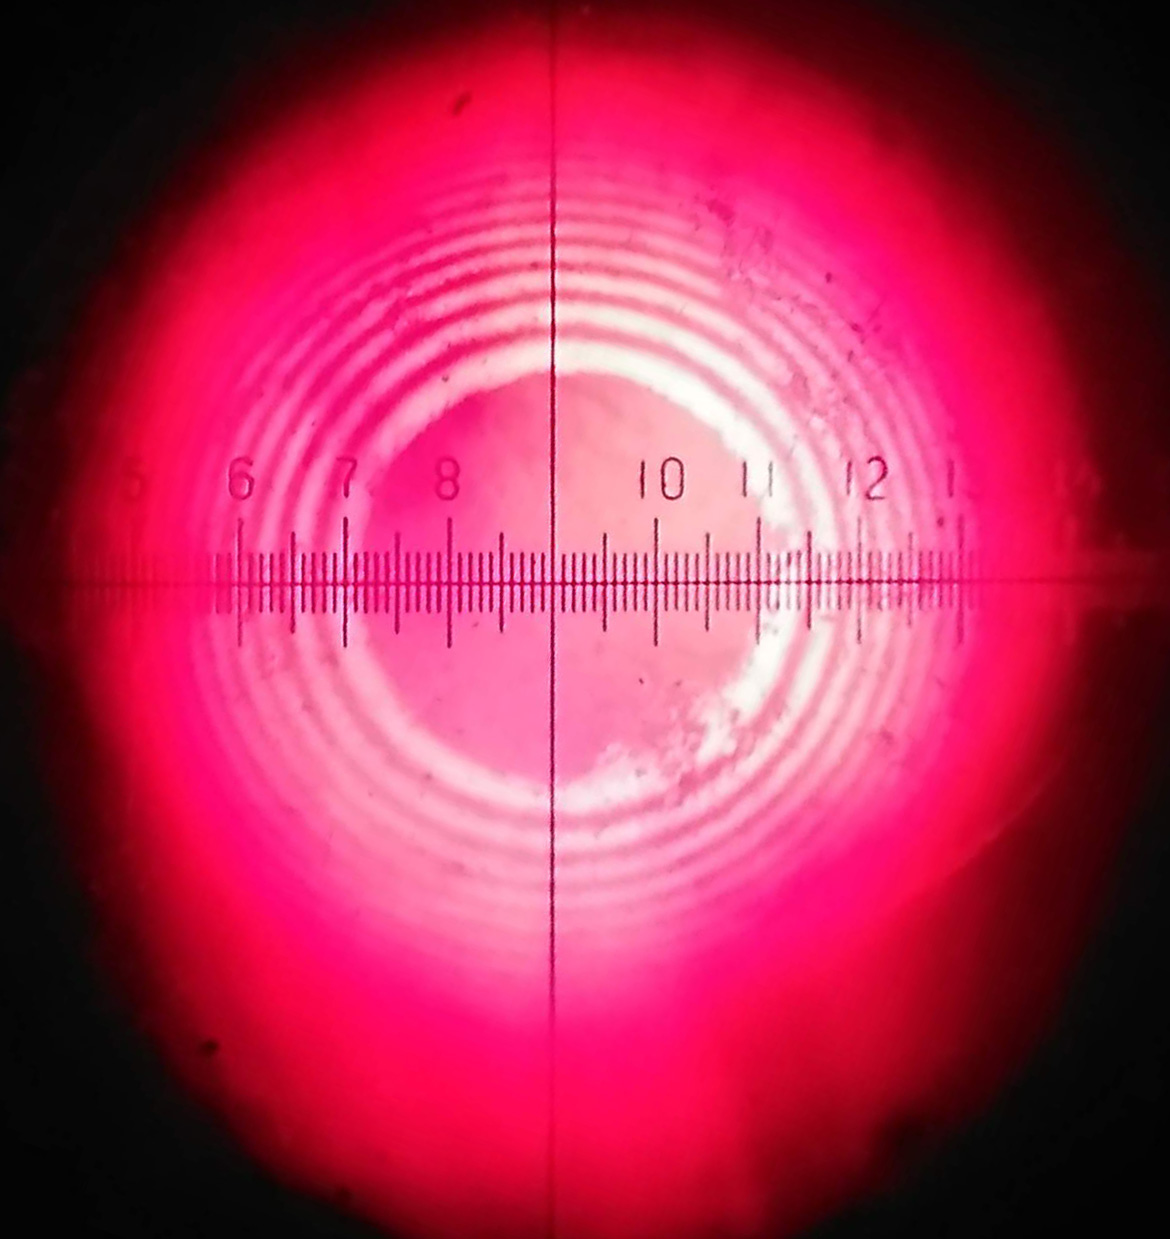
\includegraphics[width=0.95\linewidth]{Red}
    \label{fig:Red}
    \end{center}
\end{minipage}%
\qquad%---------------------------------------------------------
\begin{minipage}{0.4\linewidth}\centering
               Експериментальні дані для червоного кольору
            \pgfplotstabletypeset[
            columns={N,r,rError,rsqr},
            columns/N/.style={int detect, column type=r, column name=$N$},
            columns/r/.style={column type=c, column name={$r$, мм}},
            columns/rError/.style={column type=c, column name={$\pm\Delta r$, мм}},
            columns/rsqr/.style={column type=c, column name={$r^2$, мм$^2$}},
            every head row/.style={
            before row=\toprule,after row=\midrule},
            every last row/.style={
            after row=\bottomrule},
             fixed, fixed zerofill,
            ]
            \RedTable
\end{minipage}

%---------------------------------------------------------
\begin{minipage}{0.4\linewidth}\centering
   \begin{center}
        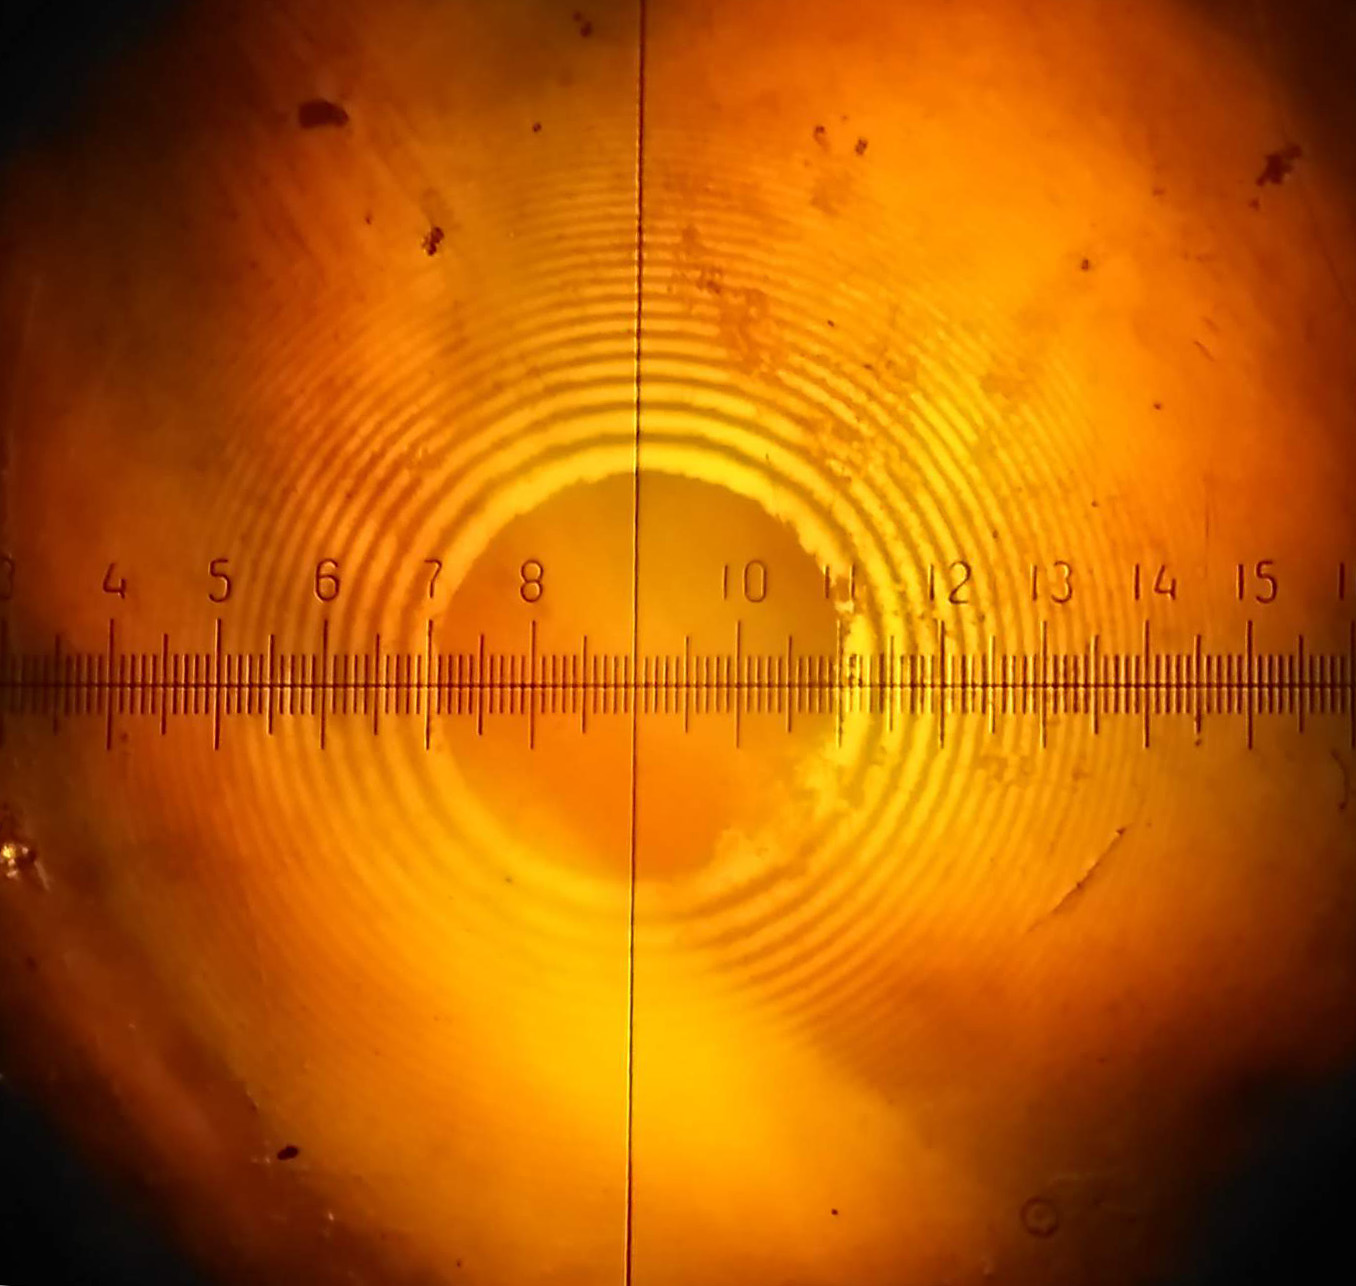
\includegraphics[width=0.95\linewidth]{Yellow}
    \label{fig:Yellow}
    \end{center}
\end{minipage}%
\qquad%---------------------------------------------------------
\begin{minipage}{0.4\linewidth}\centering
               Експериментальні дані для жовтого кольору
            \pgfplotstabletypeset[
            columns={N,r,rError,rsqr},
            columns/N/.style={int detect, column type=r, column name=$N$},
            columns/r/.style={column type=c, column name={$r$, мм}},
            columns/rError/.style={column type=c, column name={$\pm\Delta r$, мм}},
            columns/rsqr/.style={column type=c, column name={$r^2$, мм$^2$}},
            every head row/.style={
            before row=\toprule,after row=\midrule},
            every last row/.style={
            after row=\bottomrule},
             fixed, fixed zerofill,
            ]
            \YellowTable
\end{minipage}

%---------------------------------------------------------
\begin{minipage}{0.4\linewidth}\centering
   \begin{center}
        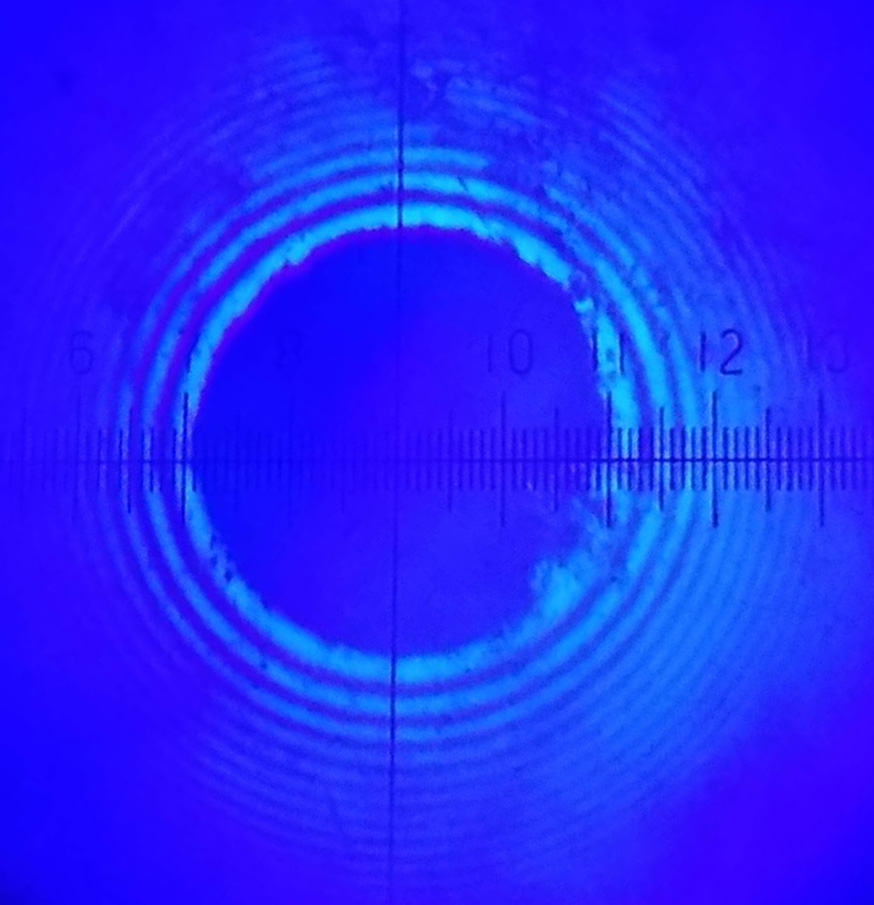
\includegraphics[width=0.95\linewidth]{Blue}
    \label{fig:Blue}
    \end{center}
\end{minipage}%
\qquad%---------------------------------------------------------
\begin{minipage}{0.4\linewidth}\centering
               Експериментальні дані для синього кольору
            \pgfplotstabletypeset[
            columns={N,r,rError,rsqr},
            columns/N/.style={int detect, column type=r, column name=$N$},
            columns/r/.style={column type=c, column name={$r$, мм}},
            columns/rError/.style={column type=c, column name={$\pm\Delta r$, мм}},
            columns/rsqr/.style={column type=c, column name={$r^2$, мм$^2$}},
            every head row/.style={
            before row=\toprule,after row=\midrule},
            every last row/.style={
            after row=\bottomrule},
             fixed, fixed zerofill,
            ]
            \BlueTable
\end{minipage}

\begin{center}
	\begin{tikzpicture}[
			declare function={
					lambdar  = 660e-6; %lambdar  = 706e-6;
                    lambday  = 620e-6; %lambday  = 585e-6;
                    lambdab  = 480e-6; %lambdab  = 404e-6;
				},
		]


		\begin{axis}[legend style={at={(current axis.north west)},anchor=north west},
				% === Налаштування сітки ===
				grid = both,
				major grid style={line width=.6pt,draw=brown!60},
				minor tick num = 9,
				minor grid style = {line width=.1pt,draw=brown!20},
%				axis lines = middle,
%				axis line style={-stealth},
				xlabel={$m$},
				ylabel={$r^2$, мм$^2$},
%				ylabel style={above right},
				every tick/.style={black},
				extra x ticks={1, 2, 3, 4, 5},
				xtick = {},
                xticklabels={},
				ytick = {},
				xmin = 1.5,
				xmax =  5.5,
				ymin = 0.3,
				ymax =  0.75,
				width=1\linewidth,
				height=0.5\textheight,
			]


			\addplot[
				red,
				only marks,
				error bars/.cd,
				y dir = both,  y explicit,
			]
			table[
					x=N,
					y expr={\thisrow{rsqr}},
					y error = rsqrError,
				]\RedTable;


			\addlegendentry{Червоний}


			\addplot[red, dashed,
			]
			table[x=N, y={create col/linear regression={y = rsqr}}]\RedTable;
			\xdef\slopeR{\pgfplotstableregressiona}
			\xdef\ycepteR{\pgfplotstableregressionb}

			\addlegendentry{
				$\pgfmathprintnumber{\slopeR} m \pgfmathprintnumber[print sign]{\ycepteR}$ ---лінійна апроксимація
			}
%-------------------------------------------------------

			\addplot[
				brown,
				only marks,
				error bars/.cd,
				y dir = both,  y explicit,
			]
			table[
					x=N,
					y expr={\thisrow{rsqr}},
					y error = rsqrError,
				]\YellowTable;

            \addlegendentry{Жовтий}

			\addplot[red, dashed,
			]
			table[x=N, y={create col/linear regression={y = rsqr}}]\YellowTable;
			\xdef\slopeY{\pgfplotstableregressiona}
			\xdef\ycepteY{\pgfplotstableregressionb}

			\addlegendentry{
				$\pgfmathprintnumber{\slopeY} m \pgfmathprintnumber[print sign]{\ycepteY}$ ---лінійна апроксимація
			}

%-------------------------------------------------------

			\addplot[
				blue,
				only marks,
				error bars/.cd,
				y dir = both,  y explicit,
			]
			table[
					x=N,
					y expr={\thisrow{rsqr}},
					y error = rsqrError,
				]\BlueTable;

            \addlegendentry{Синій}

			\addplot[blue, dashed,
			]
			table[x=N, y={create col/linear regression={y = rsqr}}]\BlueTable;
			\xdef\slopeB{\pgfplotstableregressiona}
			\xdef\ycepteB{\pgfplotstableregressionb}

			\addlegendentry{
				$\pgfmathprintnumber{\slopeB} m \pgfmathprintnumber[print sign]{\ycepteB}$ ---лінійна апроксимація
			}

% ----------------------------------------------------------------------------------------------------------
			\node[anchor = south east, text width=5cm] at (current axis.south east) {
				\begin{tornpage}
					$\lambda_{Red} = \pgfmathprintnumberFE[custom exponent=-6,precision=2]{lambdar}$~мм \\
					$R = \pgfmathprintnumberFE[custom exponent=0, precision=1, fixed zerofill]{\slopeR/lambdar/10} \pm
                    \pgfmathprintnumberFE[custom exponent=0,precision=1]{1/lambdar/10*sqrt(0.005^2+\slopeR^2*1e-10/lambdar^2)}$~см \\
                    \hrulefill\\
					$\lambda_{Yellow} = \pgfmathprintnumberFE[custom exponent=-6,precision=2]{lambday}$~мм \\
					$R = \pgfmathprintnumberFE[custom exponent=0, precision=1, fixed zerofill]{\slopeY/lambday/10} \pm
                    \pgfmathprintnumberFE[custom exponent=0,precision=1]{1/lambday/10*sqrt(0.0032^2+\slopeY^2*1e-10/lambday^2)}$~см \\
                    \hrulefill \\
					$\lambda_{Blue} = \pgfmathprintnumberFE[custom exponent=-6,precision=2]{lambdab}$~мм \\
					$R = \pgfmathprintnumberFE[custom exponent=0, precision=1, fixed zerofill]{\slopeB/lambdab/10} \pm
                    \pgfmathprintnumberFE[custom exponent=0,precision=1]{1/lambdab/10*sqrt(0.005^2+\slopeB^2*1e-10/lambdab^2)}$~см \\
				\end{tornpage}
			};
		\end{axis}
	\end{tikzpicture}

Результати експерименту та розраховане значення радіуса кривизни лінзи $R$
\end{center}

%---------------------------------------------------------


\end{document}